\documentclass[unicode,11pt,a4paper,oneside,numbers=endperiod,openany]{scrartcl}
\usepackage{amsmath}
\usepackage{amssymb}
\usepackage{ifthen}
\usepackage[utf8]{inputenc}
\usepackage{graphics}
\usepackage{graphicx}
\usepackage{hyperref}

\pagestyle{plain}
\voffset -5mm
\oddsidemargin  0mm
\evensidemargin -11mm
\marginparwidth 2cm
\marginparsep 0pt
\topmargin 0mm
\headheight 0pt
\headsep 0pt
\topskip 0pt        
\textheight 255mm
\textwidth 165mm

\newcommand{\duedate} {}
\newcommand{\setduedate}[1]{%
\renewcommand\duedate {Due date:~ #1}}
\newcommand\isassignment {false}
\newcommand{\setassignment}{\renewcommand\isassignment {true}}
\newcommand{\ifassignment}[1]{\ifthenelse{\boolean{\isassignment}}{#1}{}}
\newcommand{\ifnotassignment}[1]{\ifthenelse{\boolean{\isassignment}}{}{#1}}

\newcommand{\assignmentpolicy}{
\begin{table}[h]
\begin{center}
\scalebox{0.8} {%
\begin{tabular}{|p{0.02cm}p{16cm}|}
\hline
&\\
\multicolumn{2}{|c|}{\Large\textbf{HPC Lab for CSE 2024 ---  Submission Instructions}}\\
\multicolumn{2}{|c|}{\large\textbf{(Please, notice that following instructions are mandatory: }}\\
\multicolumn{2}{|c|}{\large\textbf{submissions that don't comply with, won't be considered)}}\\
&\\
\textbullet & Assignments must be submitted to \href{https://moodle-app2.let.ethz.ch/course/view.php?id=22516}{Moodle} (i.e. in electronic format).\\
\textbullet & Provide both executable package and sources (e.g. C/C++ files, Matlab). 
If you are using libraries, please add them in the file. Sources must be organized in directories called:\\
\multicolumn{2}{|c|}{\textit{Project\_number\_lastname\_firstname}}\\
& and  the  file must be called:\\
\multicolumn{2}{|c|}{\textit{project\_number\_lastname\_firstname.zip}}\\
\multicolumn{2}{|c|}{\textit{project\_number\_lastname\_firstname.pdf}}\\
\textbullet &  The TAs will grade your project by reviewing your project write-up, and looking at the implementation 
                 you attempted, and benchmarking your code's performance.\\

\textbullet & You are allowed to discuss all questions with anyone you like; however: (i) your submission must list anyone you discussed problems with and (ii) you must write up your submission independently.\\
\hline
\end{tabular}
}
\end{center}
\end{table}
}
\newcommand{\punkte}[1]{\hspace{1ex}\emph{\mdseries\hfill(#1~\ifcase#1{Points}\or{Points}\else{Points}\fi)}}


\newcommand\serieheader[6]{
\thispagestyle{empty}%
\begin{flushleft}

\includegraphics[width=0.4\textwidth]{ETHlogo_13}
\end{flushleft}
  \noindent%
  {\large\ignorespaces{\textbf{#1}}\hspace{\fill}\ignorespaces{ \textbf{#2}}}\\ \\%
  {\large\ignorespaces #3 \hspace{\fill}\ignorespaces #4}\\
  \noindent%
  \bigskip
  \hrule\par\bigskip\noindent%
  \bigskip {\ignorespaces {\Large{\textbf{#5}}}
  \hspace{\fill}\ignorespaces \large \ifthenelse{\boolean{\isassignment}}{\duedate}{#6}}
  \hrule\par\bigskip\noindent%  \linebreak
 }

\makeatletter
\def\enumerateMod{\ifnum \@enumdepth >3 \@toodeep\else
      \advance\@enumdepth \@ne
      \edef\@enumctr{enum\romannumeral\the\@enumdepth}\list
      {\csname label\@enumctr\endcsname}{\usecounter
        {\@enumctr}%%%? the following differs from "enumerate"
	\topsep0pt%
	\partopsep0pt%
	\itemsep0pt%
	\def\makelabel##1{\hss\llap{##1}}}\fi}
\let\endenumerateMod =\endlist
\makeatother




\usepackage{textcomp}






\begin{document}


\setassignment
\setduedate{Monday 20 May 2024, 23:59}

\serieheader{AI in the Sciences and Engineering}{Spring Semester 2024}
            {Student: Carla Judith L\'opez Zurita}
            {}{Project 2}{}
\newline

The main objective of the project is to apply the concepts learned in class
related to Neural Operators. 
The first task consists in making future (or out of samples) predictions of the fluid and solid
temperature of a thermal storage system. The second task is to model the water
flow on the sphere using a
Spherical Fourier Neural Operator (SFNO) and compare the results with the ones
obtained by a baseline neural operator.
The project also includes an optional task to test the universal approximation
property of the Convolutional Neural Operator (CNO).
My attempt at solving each of the mentioned tasks will be described in detail below.


\section{Time Series Forecasting with Neural Operators}\label{sec:task1}
The first task is based on the mathematical model of a thermal storage system
described by the following PDEs:
\begin{align}
    \epsilon \rho_f C_f \frac{\partial T_f}{\partial t} + \epsilon \rho_f C_f u_f(t) \frac{\partial T_f}{\partial x} = \lambda_f \frac{\partial^2 T_f}{\partial x^2} - h_v(T_f - T_s), \quad x \in [0, L], \quad t \in [0, T],
    \\
    (1-\epsilon)\rho_s C_s\frac{\partial T_s}{\partial t} = \lambda_s \frac{\partial^2 T_s}{\partial x^2} + h_v(T_f - T_s),  \quad x \in [0, L], \quad t \in [0, T],
\end{align}
with $\rho$ the density of the phases, $C$ the specific heat, $\lambda$ the diffusivity, $\epsilon$ the solid porosity, $u_f$
the fluid velocity entering the thermal storage and $h_v$ the heat exchange
coefficient.
The system is also defined with appropriate boundary conditions defined in the
project description.
The goal is to predict the fluid and solid temperature at future time steps
using a Neural Operator.
One of the main challenges of this task was to arrange the data in the correct
format to feed it to the network, namely the data had to be arranged in a
series of windows. I used a window generator to create the windows with a length
of 34 for both inputs and outputs, which was chosen because it is the size of the
final target prediction. 
The outputs were taken from the provided measurements, each  corresponding to the
next 34 time steps of a given time. Fig. \ref{fig:window} shows an example of a
window with its 
prediction.
\begin{figure}[ht!]
    \centering
    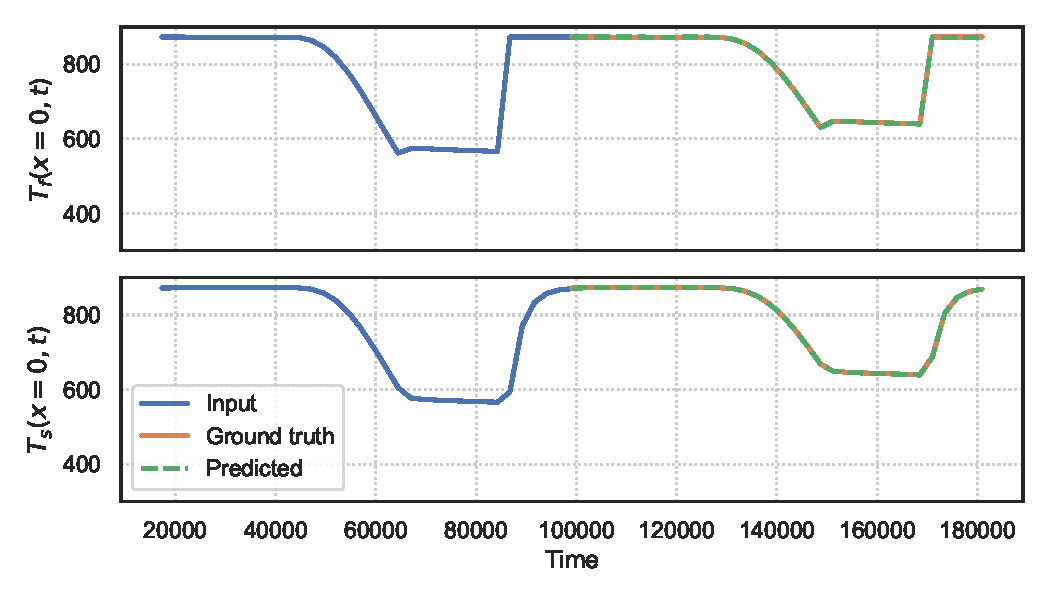
\includegraphics[width=0.8\textwidth]{../task1/fno/plot_window_5.pdf}
    \caption{Example of a window with prediction.}
    \label{fig:window}
\end{figure}

The data was normalized using the MinMaxScaler from the sklearn library.
The data was split into training and validation sets with a
ratio of 80\% and 20\%.
I chose to use a Fourier Neural Operator (FNO) to solve this task. I used a
single network to predict both the fluid ($T_f$) and solid temperature ($T_s$),
so that it had three
channels as inputs ($T_f$, $T_s$ and time) and two channels as outputs ($T_f$ and
$T_s$). 
The network
consisted of 3 layers with 3 Fourier features each.
It was trained using the Adam optimizer with an initial learning rate
of $10^{-3}$ and a batch size of 10. 
The learning rate was adjusted using \texttt{StepLR} with step size of 50 and gamma 0.5.
The loss function used was the L2 norm and it was trained for 1,000 epochs,
which tool around two minutes on a single core, in a M1 MacBook Pro.
The loss function of the model during training is shown in Fig. \ref{fig:loss}.
\begin{figure}[ht!]
    \centering
    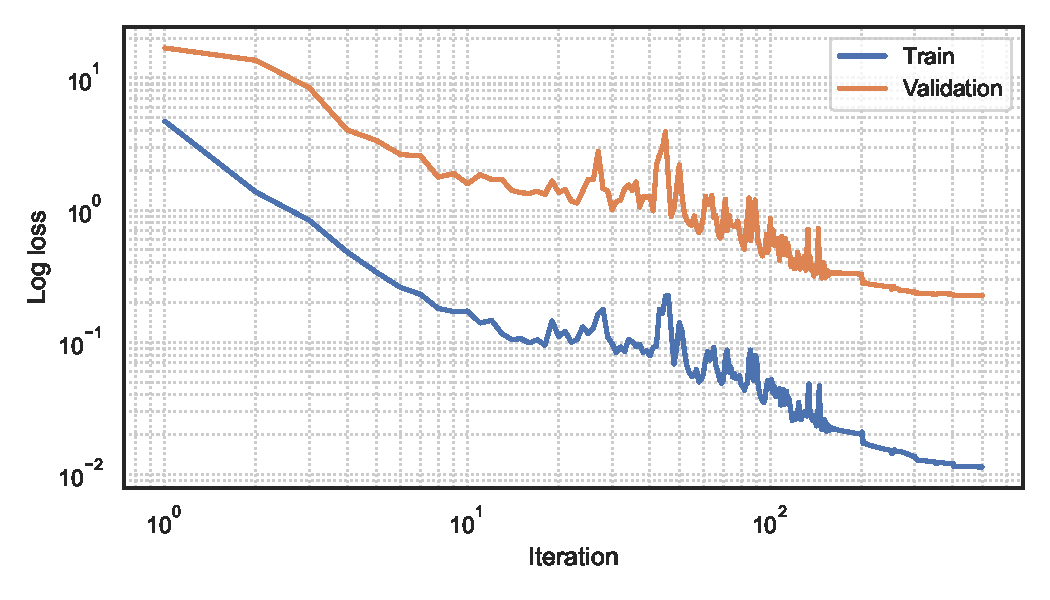
\includegraphics[width=0.8\textwidth]{../task1/fno/loss_function.pdf}
    \caption{Loss function of the FNO model during training.}
    \label{fig:loss}
\end{figure}

The model was evaluated on the test set and the predictions were compared with
the ground truth. Fig. \ref{fig:predictions} shows the predictions of the model
taken from various windows in the test set.
The model seems to be able to capture the general trend of the data, and predict
very close values.
\begin{figure}[ht!]
    \centering
    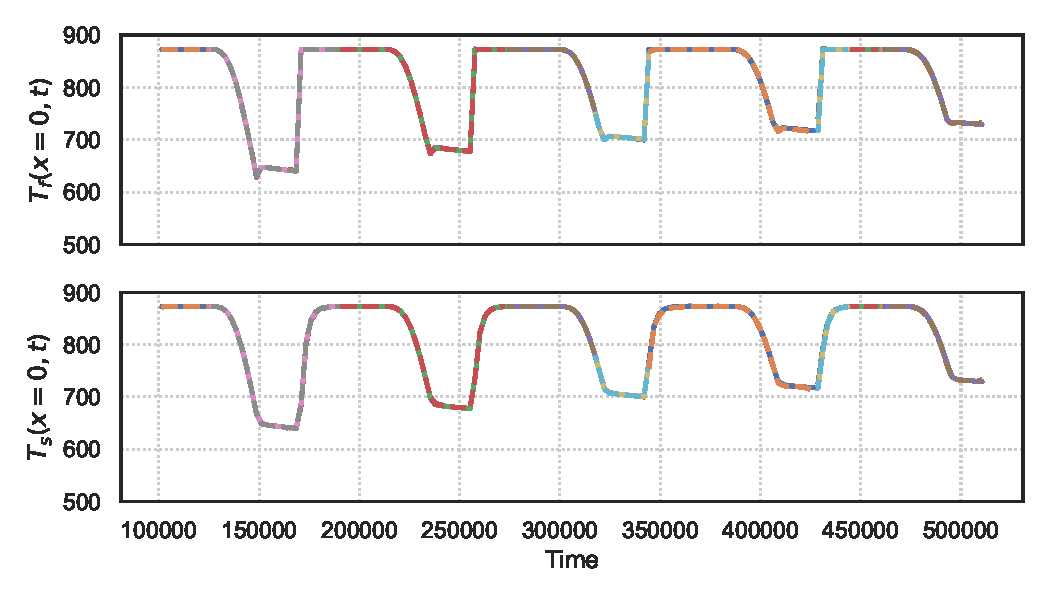
\includegraphics[width=0.8\textwidth]{../task1/fno/plot_predictions.pdf}
    \caption{Predictions of the FNO model taken from various windows in the test set. Dashed lines represent the predicted values, solid lines depict ground truth.}
    \label{fig:predictions}
\end{figure}

Finally, we show the future predictions of the fluid and solid temperature in
Fig. \ref{fig:future}.
\begin{figure}[ht!]
    \centering
    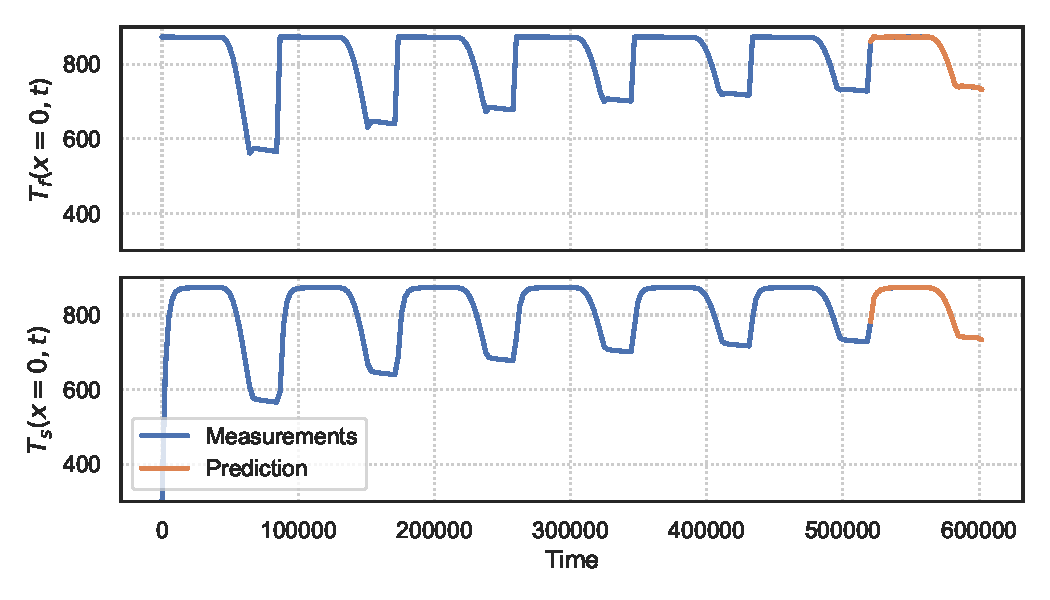
\includegraphics[width=0.8\textwidth]{../task1/fno/plot_complete.pdf}
    \caption{Future predictions of the fluid and solid temperature.}
    \label{fig:future}
\end{figure}

\section{Modeling Water Flow on the Sphere with FNO}\label{sec:task2}
The next task consists in modeling the water flow on the sphere using Neural Operators.
The idea of the task is to use two different architectures to predict the
velocity field of the water on the sphere for various resolutions while training
on a lower resolution. 
In this manner, we can see how the model generalizes to out of sample data.
We will implement an Spherical
Fourier Neural Operator (SFNO) and compare the results with those of a baseline
neural operator, in this case, a Fourier Neural Operator (FNO).
The main difference between the two models is that the SFNO uses spherical
harmonics to represent the data, while the FNO uses Fourier features. This was
implemented by building a custom layer that computes the spherical harmonics
using function from Bonev et al's library \cite{bonev2023spherical}.
The architectures were based on the paper and public code repository by Zongyi
Li et al \cite{li2020fourier}.

The data was retrieved from the Kossaifi et al's library
\cite{neuraloperator2024sfno}; it contains the velocity
field of water on the sphere, as well as the $x$ and $y$ coordinates of the
sphere.
The data was split using 200 samples for training with (32, 64) resolution and
50 samples for validation for (32, 64) and (64, 128) resolutions. It was
normalized using the StandardScaler from the sklearn library.

The FNO model was trained using Adam optimizer with an initial learning rate of
$8e^{-4}$ and a batch size of 4 for training and 10 for testing. The learning rate was adjusted using
\texttt{CosineAnnealingLR} with a $T_{\text{max}}$ of 30. 
The loss function used was the L2 norm.
The network was trained for 20 epochs, which took around 20 minutes on a single
core, in a M1 MacBook Pro. 
The loss function of the model using FNO during training is shown in Fig.
\ref{fig:loss_fno2d}.
The SFNO model was trained using the same parameters as the FNO model, and took
appropriately the same time to train. The loss function of the model using SFNO
during training is shown in Fig. \ref{fig:losss_sfno2d}.
\begin{figure}[ht!]
    \centering
    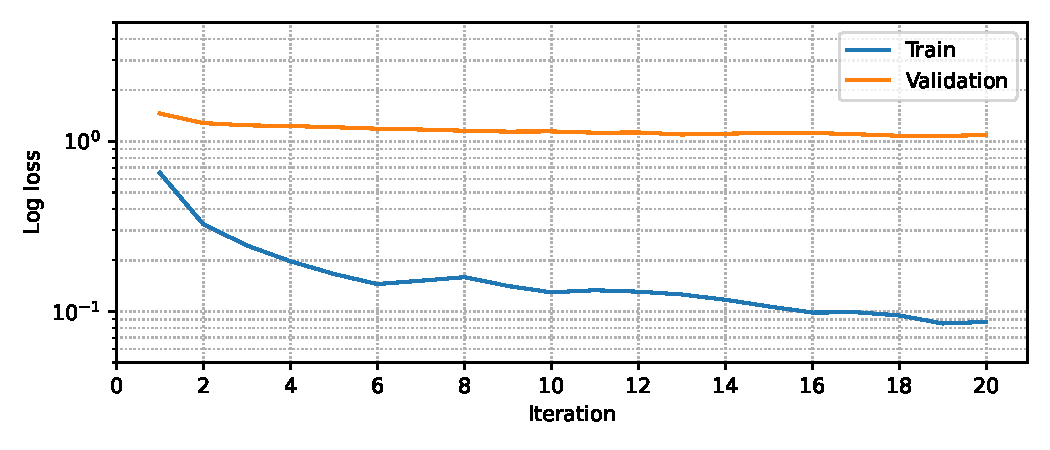
\includegraphics[width=0.8\textwidth]{../task2/sfno/loss_function_FNO2d.pdf}
    \caption{Loss function of the FNO model during training.}
    \label{fig:loss_fno2d}
\end{figure}
\begin{figure}[ht!]
    \centering
    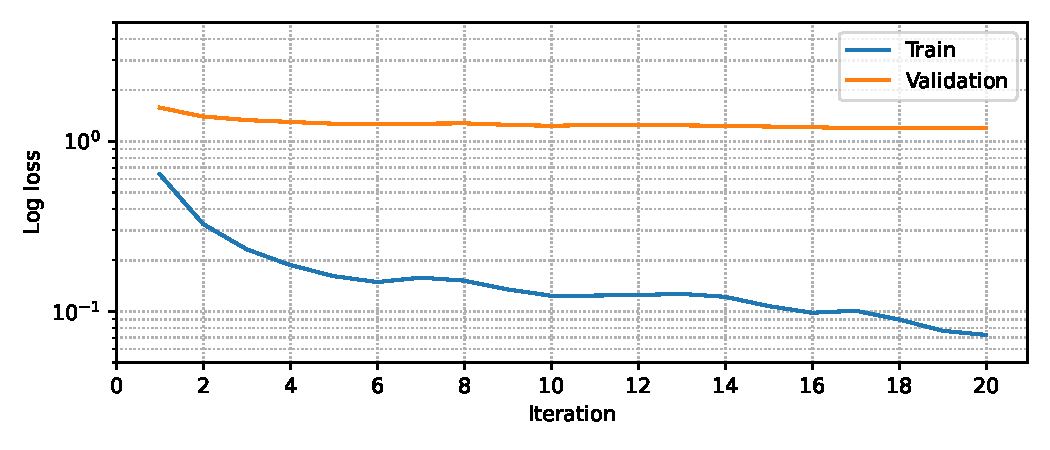
\includegraphics[width=0.8\textwidth]{../task2/sfno/loss_function_SFNO2d.pdf}
    \caption{Loss function of the SFNO model during training.}
    \label{fig:losss_sfno2d}
\end{figure}
We can see that both models converge in a similar manner, but the SFNO
model seems to reach a lower loss value in the training set, as shown in Table
\ref{tab:evaluation_metrics}.
\begin{table}[ht!]
    \centering
    \begin{tabular}{lcc}
        \hline
        \textbf{Model} & \textbf{Train Norm} & \textbf{Test Norm} \\
        \hline
        FNO & 0.086722 & 1.089633 \\
        SFNO & 0.0726737  & 1.197494 \\
        \hline
    \end{tabular}
    \caption{Value of the relative L2 norm for the FNO and SFNO model after 20 epochs.}
    \label{tab:evaluation_metrics}
\end{table}
Nevertheless, the FNO model seems to generalize better to the validation set.
It is important to mention that the loss values are directly comparable
between the two models, since the data and training was handled in the same way.
It is also reasonable to see why the values of the loss function between
training and validation sets are different, as the validation set at higher
resolution is unseen data for the model when training.
This is bound to give a higher loss value. Training for more epochs did not seem
to improve the results of both models, even as the loss function of the training
set kept decreasing, the loss function of the validation set started increasing,
which is a sign of overfitting.

Finally, we show an example of the velocity field of water on the sphere using
the FNO model in Fig. \ref{fig:example_fno2d} and the SFNO model in Fig.
\ref{fig:example_sfno2d}.
\begin{figure}[ht!]
    \centering
    \includegraphics[width=\textwidth]{../task2/sfno/results/results_4_FNO2d.png}
    \caption{Example of the velocity field of water on the sphere using a FNO.}
    \label{fig:example_fno2d}
\end{figure}
\begin{figure}[ht!]
    \centering
    \includegraphics[width=\textwidth]{../task2/sfno/results/results_1_SFNO2d.png}
    \caption{Example of the velocity field of water on the sphere using a SFNO.}
    \label{fig:example_sfno2d}
\end{figure}
Qualitatively, both models seem to capture the general trend of the data
correctly, specially in the resolution they were trained on. Both models seem to
create some aritifacts in the velocity field, and also seem to retain some more
details compared to the ground truth. It is hard to say which model is better
without further analysis.
More examples of the velocity field of water on the sphere using the FNO model
and the SFNO model can be found in the \texttt{results} folder attached to this document.

\section{Universal Approximation for CNO}\label{sec:task3}
Consider the abstract PDE in the 2d torus $D = \mathbb{T}^2$,
$\mathcal{L}(u) = 0$, $\mathcal{B}(u) = 0$,
with $\mathcal{L}$ being a differential operator and $\mathcal{B}$ a boundary operator. We assume that the differential
operator $\mathcal{L}$ only depends on the coordinate $x$ through a coefficient function
$a \in H^r(D)$. The corresponding \textit{solution} operator is denoted by 
$\mathcal{G}^{\dagger} : X^* \in H^r(D) \to H^r(D) : a \to u$, with $u$ being the
solution of the PDE. $H^r(D)$ is Sobolev space of order $r$.


We define the operator $\mathcal{G}: \mathcal{B}_w(D) \to \mathcal{B}_w(D)$ as a
convolutional neural operator (CNO) which is a compositional mapping between
functions, built as follows \cite{raonic2023convolutional}
:
\begin{align}
    \mathcal{G} :u\to P(u)=v_0 \to v_1 \to \cdots v_L \to Q(vL)=u,
\end{align}
where $P$ and $Q$ are the input and output processing functions, respectively, and $v_l$ are the intermediate feature maps. The CNO is defined as a composition of three types of operators: a convolutional operator $\mathcal{K}_l$, a non-linear activation function $\Sigma_l$ and a pointwise operator $\mathcal{P}_l$.
\begin{align}
     v_{l+1} =\mathcal{P}_l \circ
    \Sigma_l
    \circ \mathcal{K}_l(v_l), \quad 1\leq l\leq L-1.
\end{align}


The universality theorem for CNO states that for any $\epsilon > 0$ and any
sufficiently regular operator $\mathcal{G}^{\dagger}$,
there exists a CNO $G$ such that for every $a \in X^*$ with $|a|H^r(D) \leq B$
it holds,
\begin{equation}
    \|\mathcal{G}(a) - \mathcal{G}^{\dagger}(a)\|_{H^r(D)} \leq \epsilon.
\end{equation}
In practice, this means that the CNO can approximate any solution operator
$\mathcal{G}^{\dagger}$ with an arbitrary precision. This is a powerful result that shows the potential of CNOs in solving PDEs.

Apart from the condition of sufficiently regular solution operators
$\mathcal{G}^{\dagger}$, we can impose some additional regularization
constraints on $\mathcal{G}^{\dagger}$, so that the universality theorem holds.
For example, we can require that the solution operator $\mathcal{G}^{\dagger}$
is Lipschitz continuous with respect to the $L^2$ norm. This is a common
regularization constraint in practice. Raonić et al.
\cite{raonic2023convolutional} also suggest defining an alternate approximation theorem that offers explicit control over the network size and provides upper bounds on the weights.

\bibliographystyle{plain}
\bibliography{bibliography}

\end{document}
